\documentclass[dvipdfmx]{standalone}
\usepackage{tikz}

\begin{document}

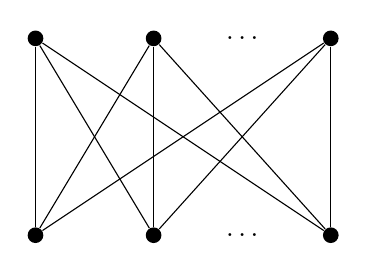
\begin{tikzpicture}
    % ===================================
    % 設定
    % ===================================
    \def\h{2.5}  % 上段と下段の距離(高さ)
    \def\w{1.5}  % 隣り合う点の間隔
    \def\sep{1.5} % ... の部分の広さ倍率
    
    \tikzset{dot/.style={circle, fill=black, inner sep=2pt}}
    % ===================================

    % 1. 上段の点の配置 (点 点 ... 点)
    \node[dot] (u1) at (0, \h) {};
    \node[dot] (u2) at (\w, \h) {};
    
    % 省略記号
    \node at (\w + \w*\sep*0.5, \h) {$\dots$};
    
    % 右端の点
    \node[dot] (un) at (\w + \w*\sep, \h) {};


    % 2. 下段の点の配置 ( 点 ... 点)
    % バランスよく配置するため、上段と同じx座標に置きます
    \node[dot] (v1) at (0, 0) {};
    % 下段も「点...点」の並びを表現するため、2つ目を配置
    \node[dot] (v2) at (\w, 0) {}; 
    
    % 省略記号
    \node at (\w + \w*\sep*0.5, 0) {$\dots$};
    
    % 右端の点
    \node[dot] (vn) at (\w + \w*\sep, 0) {};


    % 3. 全ての点同士を辺で結ぶ
    % 上段の点リスト
    \foreach \u in {u1, u2, un} {
        % 下段の点リスト
        \foreach \v in {v1, v2, vn} {
            \draw (\u) -- (\v);
        }
    }

\end{tikzpicture}

\end{document}